% !TeX spellcheck = en_US

\chapter{Groundwork}
This chapter covers the basic technologies and term used throughout the following chapters.



\section{MARS Websuite}
The MARS Websuite is the web application of the MARS working group. It allows the user to prepare and start simulation runs from within the web browser.\\
The original Websuite has a monolithic structure, meaning it is a traditional, single application with many responsibilities, parts and technologies. The new Websuite contains of over 20 independent microservices.\\
This work focuses on extracting the front-end of the fullstack application into a single microservice. While doing so, the inherited components are to be reevaluated, redesigned and if needed, rewritten.



\section{Microservices}
\label{sec:microservices}
Microservices describes a software architecture, where the software is split up into small, independent components. These components are loosely coupled and communicate over the network. Each so called service runs in its own process and potentially on a different machine.


\subsection{Single responsibility}
Big, monolithic application grow in size and complexity during their existing. This resolves into higher costs for maintenance and enhancements. Microservices reduce complexity by splitting the application into smaller logical parts. The definition of \enquote{micro} varies. \cite{newman2015building} e.g. claims that microservices should follow the \enquote{Single responsibility principle} by \cite{martin2003agile}. This states that a given component should have only one reason to change.


\subsection{Autonomy}
Each microservice is deployed its own process. The processes communicate with each other via a RESTful API. It is therefore possible to scale up single services as needed, without having to scale the whole application.\\
Communication between services are no local system calls, like in a monolithic application. This means, that the communication partner is within a different trust boundary and potentially in a different network. Microservice therefore have to be built with resilience, so their capability to work does not depend on other services.


\subsection{History}
The concept of handling growing complexity in software is not a new one. The first known approach goes back to Conway's law \cite{conway1968committees}. Conway claims that interfaces should reflect social boundaries within an organization.\\
A more recent approach towards handling complexity is Service-Oriented Architecture (SOA) by \cite{as2005service}. SOA is described as an architecture, were independent services communicate with each other over the network.\\
The term microservices was introduced by \cite{martinfowler2014microservices}. Their approach is a more specific version of SOA. This is why microservices are often referred to as \enquote{SOA done right}.\\
The rise of containerization software like docker, allows to deploy and run services without a substantial overhead. This strongly increased the popularity of microservices over the last 2 years.



\section{AngularJS}
\label{sec:angularjs}
The front-end is written with the JavaScript framework AngularJS v1.5. AngularJS was created by Miško Hevery at Brat Tech LLC in the year 2010 and is under active development by Google Inc. \\
The framework extends HTML5 and JavaScript by various paradigms and patterns. This makes the development of single-page web applications more appealing. The most relevant features are the \textit{Templating Engine}, \textit{Two Way Data-Binding}, \textit{Model–view–viewmodel} and \textit{Dependency Injection}.


\subsection{Template Engine}
The Angular template is responsible for rendering the logic from the JavaScript controller into the HTML. This is either done by the curly braces syntax which wraps the expression into double curly braces or by custom HTML tags, called directives.\vspace{1ex}

\noindent\textbf{Directives} -- Are Angular's method of extending HTML by new elements with JavaScript logic attached. This can be used to create reusable, parameterized components.\vspace{1ex}

\noindent\textbf{Markup} -- Variables from the controller can be referenced by the double curly brackets notation.\vspace{1ex}

\noindent\textbf{Filter} -- Angular has build-in filters to reduce or format a given expression. Amongst others, this can be used to format numbers as currency or make a JSON output more readable.\vspace{1ex}

\noindent\textbf{Form controls} --Allows validation of formdata. A field marked as required hat an error CSS class attached, as well as a JavaScript class that allows to easily validate user input.


\subsection{Two Way Data-Binding}
\label{sec:tw-binding}
Data in Angular is bound to a Model, which always holds the most recent state of the application. Changes to the data are always passed to the model and read from it. This means that the controller and the view always have the same state of the data. The need to write boilerplate code, for transferring states between the HTML view and the JavaSript controller is hereby removed. Figure \ref{fig:tw-databinding} emphasizes this.

\begin{figure}[H]
	\centering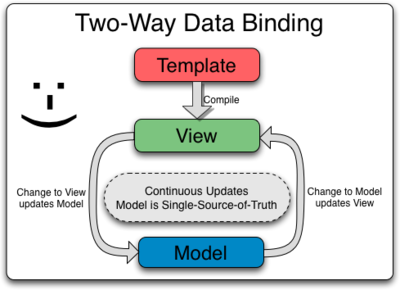
\includegraphics[width=0.5\textwidth]{res/Two_Way_Data_Binding}
	\caption{AngularJS two-way data binding: \url{https://docs.angularjs.org/guide/databinding}}
	\label{fig:tw-databinding}
\end{figure}


\subsection{Model–view–viewmodel (MVVM)}
Angular takes advantage of the Model View Controller (MVC) pattern. The implementation however is closer to an Model–view–viewmodel (MVVM) approach. 

\subsubsection{Model}
The Model in Angular is responsible for storing the current state of the application. Since the model is a simple JavaScript object, no boilerplate for getting and setting data is necessary.

\subsubsection{ViewModel}
The ViewModel is an object that manages specific views and stores the data that is passed between the Controller and the View. In the past, this was done, by injecting \$scope into the controller. Since Angular 1.5 the recommended way is to create a ViewModel variable like shown in listing \ref{lst:angular}.

\subsubsection{Controller}
The Controller sets the initial state of the ViewModel and adds values and functions to it. This added functionality defines the behavior of the application. It is worth noting that the Controller does not store any state and that it is not responsible for the communication between services.

\subsubsection{View}
The View is the HTML, that exists, once Angular has interpreted the template and the appertaining data.

\subsection{Dependency Injection (DI)}
AngularJS brings dependency injection support to JavaScript. It allows the integration of global available dependencies into a specific controller. This ensures the availability of a component to specific controllers only.\\
It is hereby possible to use existing parts, as well as create own modules that can be used anywhere throughout application. The decoupling of components prevents the necessity for duplicate code and makes it easy to pull in 3rd party dependencies.  

\subsection{Example}
The following example takes advantage of the concepts mentioned in the sections above. It shows a simple Angular application that defines a \textit{Fruits} factory, injects it into a controller and uses the ng-repeat directive to iterate over the content. Inside the loop the current fruit is rendered to a list, using the double curly brackets notation.

\begin{lstlisting}[language=javascript, caption=AngularJS directive and controller definition, label=lst:angular]
angular.module("myApp", [])
  .factory('Fruits', function() {
    return {
      get: function() {
        return ["apple", "orange", "raspberry"];
      }
    };
  })
  
  .controller("FruitController", function(Fruits) { // inject Fruits
    var vm = this; // ViewModel
    vm.fruits = Fruits.get(); // call directive
  });
\end{lstlisting}

\begin{lstlisting}[language=html, caption=AngularJS template]
<div ng-app="myApp" ng-controller="FruitController as fruitCtrl">
  <ul>
    <li ng-repeat="fruit in fruitCtrl.fruits">
      {{fruit}}
    </li>
  </ul>
</div>
\end{lstlisting}

\begin{lstlisting}[language=html, caption=HTML result]
<ul>
  <li>apple</li>
  <li>orange</li>
  <li>raspberry</li>
</ul>
\end{lstlisting}


\subsection{Angular2}
On September 14th 2016, Angular 2 stable was first released. Version 2 is a complete rewrite of the original AngularJS implementation and therefore offers no direct update path.\\
When the MARS Websuite was first developed, Angular 2 was not an option. Right now, there are no plans, to port the application to the new version, since the migration would involve rewriting substantial parts of the application. This is why Angular2 will not be covered in this work.
